\section{eo\-Truncated\-Select\-One$<$ EOT $>$ Class Template Reference}
\label{classeo_truncated_select_one}\index{eoTruncatedSelectOne@{eoTruncatedSelectOne}}
eo\-Truncated\-Select\-One selects one individual using {\bf eo\-Select\-One}{\rm (p.\,\pageref{classeo_select_one})} as it's mechanism.  


{\tt \#include $<$eo\-Truncated\-Select\-One.h$>$}

Inheritance diagram for eo\-Truncated\-Select\-One$<$ EOT $>$::\begin{figure}[H]
\begin{center}
\leavevmode
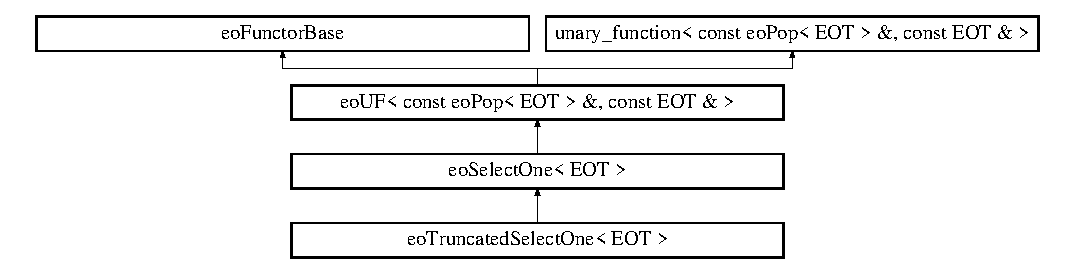
\includegraphics[height=3.23699cm]{classeo_truncated_select_one}
\end{center}
\end{figure}
\subsection*{Public Member Functions}
\begin{CompactItemize}
\item 
{\bf eo\-Truncated\-Select\-One} ({\bf eo\-Select\-One}$<$ {\bf EOT} $>$ \&\_\-select, double \_\-rate\-Fertile, bool \_\-interpret\_\-as\_\-rate\-F=true)\label{classeo_truncated_select_one_a0}

\begin{CompactList}\small\item\em Ctor from rate and bool. \item\end{CompactList}\item 
{\bf eo\-Truncated\-Select\-One} ({\bf eo\-Select\-One}$<$ {\bf EOT} $>$ \&\_\-select, {\bf eo\-How\-Many} \_\-how\-Many\-Fertile)\label{classeo_truncated_select_one_a1}

\begin{CompactList}\small\item\em Ctor with {\bf eo\-How\-Many}{\rm (p.\,\pageref{classeo_how_many})}. \item\end{CompactList}\item 
void {\bf setup} (const {\bf eo\-Pop}$<$ {\bf EOT} $>$ \&\_\-source)\label{classeo_truncated_select_one_a2}

\begin{CompactList}\small\item\em setup procedures: fills the temporary population with the fertile guys \item\end{CompactList}\item 
const {\bf EOT} \& {\bf operator()} (const {\bf eo\-Pop}$<$ {\bf EOT} $>$ \&\_\-pop)
\begin{CompactList}\small\item\em The implementation selects an individual from the fertile pop. \item\end{CompactList}\end{CompactItemize}
\subsection*{Private Attributes}
\begin{CompactItemize}
\item 
{\bf eo\-Select\-One}$<$ {\bf EOT} $>$ \& {\bf select}\label{classeo_truncated_select_one_r0}

\item 
{\bf eo\-How\-Many} {\bf how\-Many\-Fertile}\label{classeo_truncated_select_one_r1}

\item 
{\bf eo\-Pop}$<$ {\bf EOT} $>$ {\bf tmp\-Pop}\label{classeo_truncated_select_one_r2}

\item 
{\bf eo\-Pop}$<$ {\bf EOT} $>$ \& {\bf actual\-Pop}\label{classeo_truncated_select_one_r3}

\end{CompactItemize}


\subsection{Detailed Description}
\subsubsection*{template$<$class EOT$>$ class eo\-Truncated\-Select\-One$<$ EOT $>$}

eo\-Truncated\-Select\-One selects one individual using {\bf eo\-Select\-One}{\rm (p.\,\pageref{classeo_select_one})} as it's mechanism. 

Therefore eo\-Truncated\-Select\-One needs an {\bf eo\-Select\-One}{\rm (p.\,\pageref{classeo_select_one})} in its ctor

It will perform selection only from the top guys in the population. 



Definition at line 45 of file eo\-Truncated\-Select\-One.h.

\subsection{Member Function Documentation}
\index{eoTruncatedSelectOne@{eo\-Truncated\-Select\-One}!operator()@{operator()}}
\index{operator()@{operator()}!eoTruncatedSelectOne@{eo\-Truncated\-Select\-One}}
\subsubsection{\setlength{\rightskip}{0pt plus 5cm}template$<$class EOT$>$ const {\bf EOT}\& {\bf eo\-Truncated\-Select\-One}$<$ {\bf EOT} $>$::operator() (const {\bf eo\-Pop}$<$ {\bf EOT} $>$ \& {\em \_\-pop})\hspace{0.3cm}{\tt  [inline, virtual]}}\label{classeo_truncated_select_one_a3}


The implementation selects an individual from the fertile pop. 

\begin{Desc}
\item[Parameters:]
\begin{description}
\item[{\em \_\-source}]the source population \item[{\em \_\-dest}]the selected guy \end{description}
\end{Desc}


Implements {\bf eo\-UF$<$ const eo\-Pop$<$ EOT $>$ \&, const EOT \& $>$} {\rm (p.\,\pageref{classeo_u_f_a1})}.

Definition at line 98 of file eo\-Truncated\-Select\-One.h.

The documentation for this class was generated from the following file:\begin{CompactItemize}
\item 
eo\-Truncated\-Select\-One.h\end{CompactItemize}
